\chapter{Task 3}
\begin{parlist}
	\item
	\begin{table}[hbt]
\centering
\caption{Table1}
\resizebox{\linewidth}{!}{%
\begin{tabular}{|l|l|} 
\hline
Use Case       & Webshop                                                                                                                                                                                                                                                                                                                                                                                                                                                                                                                                         \\ 
\hline
Description    & A company wants to use the Database in a webshop to check if they can sell a product to a customer                                                                                                                                                                                                                                                                                                                                                                                                                                              \\ 
\hline
Actors         & Customer company-employee/website                                                                                                                                                                                                                                                                                                                                                                                                                                                                                                               \\ 
\hline
Assumptions    & The product data is stored in the database, the data in the database is accurate                                                                                                                                                                                                                                                                                                                                                                                                                                                                \\ 
\hline
Steps          & \begin{tabular}{@{}l@{}}{\labelitemi}\hspace{\dimexpr\labelsep+0.5\tabcolsep}Webserver recieves purchase request\\{\labelitemi}\hspace{\dimexpr\labelsep+0.5\tabcolsep}Webserver sends query to database\\{\labelitemi}\hspace{\dimexpr\labelsep+0.5\tabcolsep}IF stock of the requested product is greater than 1\\\hspace{0.5\leftmargin}{\labelitemii}\hspace{\dimexpr\labelsep+0.5\tabcolsep}THEN~webserver continues purchasing process\\{\labelitemi}\hspace{\dimexpr\labelsep+0.5\tabcolsep}ELSE~webserver rejects request\end{tabular}  \\ 
\hline
Variation      & The webserver could check if the user has already bought x of the product and reject their offer according to a x per person policy                                                                                                                                                                                                                                                                                                                                                                                                             \\ 
\hline
Non-Functional & The database must be able to handle multiple queries at once in order to process multiple orders at once                                                                                                                                                                                                                                                                                                                                                                                                                                        \\ 
\hline
Issues         &                                                                                                                                                                                                                                                                                                                                                                                                                                                                                                                                                 \\
\hline
\end{tabular}
}
\end{table} 
	\item
	 \begin{figure}[hbt]
	 	\label{fig1}
		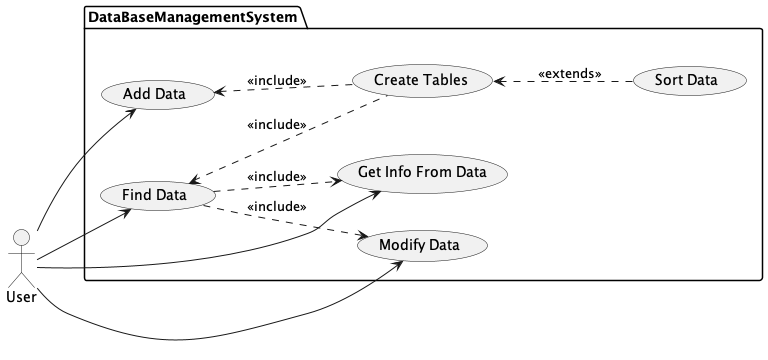
\includegraphics[width=\textwidth]{Immagini/test.png}
	  \caption{UMl-UseCase}
\end{figure}

\end{parlist}
